\chapter{Optical Enhancement of Core-Shell Nanowire} \label{data}

Given that the profound enhancement of optoeletronic properties of nanowires is
the major theme of this dissertation, it is dutiful to first summarize the
major experimental results, such as fabrication and characteristics of
core-shell nanowires (CSNWs).

Electron systems in lower dimensions are adequately treated through
perturbation methods. For 1D electron systems (1DES) the correlations among
electrons are much more significant due to higher degrees of confinement. The
electron can either be moving to the left or right and any small or localized
interaction can cause a collective response from the whole system. This is the
condition of broken symmetry, in which the overall status of the system has to
be reformulated. For a 2DES, a broken symmetry occurs at very low densities of
fermions, in which formation of a Wigner lattice is expected, which is due to
the Coulombic interactions of electrons. Interestingly for a 1DES, the
direction of movement for fermions is restricted to the left or right.
Consequently, the density of the system becomes irrelevant with respect to the
determination of the status of the system. Such a 1D many electron system is
often called a $L\ddot{u}finger$ Liquid, as he was the first person who
successfully formulated these systems.

Importantly, a 1DES can experimentally be realized in various material systems.
These include carbon nanotubes, electrons at the edges of a 2DES, and in
nanowires.

A core-shell nanowire (CSNW) is a quasi-one dimensional structure with a wide
band gap materials, such as AlGaAs, wrapping around a low band gap
semiconductor, such as GaAs.

It is expected that the lower dimensionality in CSNW to have a significant
influence on both optical and electrical properties of the structure. Fot
instantce,

Electrically it is important account for the electron correlations in order to
determine the behavior of the structure. The significant values of exchange
and correlation energies in 1DES, makes them an interesting candidate for
probing their energy dynamics. This, however, imposes various experimental
challenges and theoretical considerations and are deferred to future
investigations.

\section{Growth of Nanowires}

Freestanding quasi-one-dimensional semiconductor nanostructures (nanowires)
based on III-V compound semiconductors, owing to their unique physical
properties, are considered ideal building blocks for the realization of
photonic and electronic nanodevices.

Currently, two bottom-up approaches to the fabrication of freestanding
nanowires are considered: (i) selective area epitaxy
(SAE)~\cite{motohisa2004catalyst} and (ii) metal-catalyst assisted grouth
through the so-called vapor-liquid-solid (VLS) mechanism~\cite{wagner1964vapor,
givargizov1975fundamental}. The latter method relies on the alloying of a metal
catalyst (usually Au) nanoparticle with the semiconductor constituent elements,
supplied through a vapor phase. The as-formed alloy acts as an initial
nucleation site for the material and further guides the nanowire growth, the
diameter of the nanowire being controlled by that of the metal nanoparticle.

An advantage of the VLS method over SAE is that it does not require
nanolithograpic processing of the substrate; furthermore, it is compatible with
most advanced epitaxial grouth techniques for III-V compounds, such as
molecular beam epitaxy, chemical beam epitaxy, and metalorganic vapor phase
epitaxy (MOVPE). 

GaAs nanowires were grown by low (50mbar) pressure MOVPE using an Aixtron
reactor model AIX200 RD. TMGa and TBAs were used as gallium and arsenic
precursors, respectively. Au nanoparticle deposited on
$(\bar{1}\bar{1}\bar{1})B$ GaAs were used to catalyze the nanowire growth. To
this purpose, VGF-grown semi-insulating (undoped) GaAs wafers oriented
$(\bar{1}\bar{1}\bar{1})B$ were used. The substrates were then first degreased
in isopropanol vapors, etched in $4H_2SO_4:1H_2O_2:2H_2O$ solution for 8 min at
around $40\,^{\circ}\mathrm{c}$, ringsed in de-ionized water and finally dried
under pure $N_2$. Au nanoparticles with $\sim 60 nm$ diameters were prepared by
reaction of $HAuCl_4$ with sodium citrate in aqueous solution and randomly
deposited on the as-prepared GaAs surface by dropping a small amount of
colloidal solution onto the substrate. The solvent (water) was then evaporated
by holding the samples on a hot plate (in air) or a few minutes; Au
nanoparticle surface densities thus achieved ranged around (1-4). 

After loading the sample into the reactor chamber, its temperature was raised,
and sample annealing was then performed for 10 min to absorb GaAs surface
oxides and organic residues originating from the Au nanoparticle synthesis.
This annealing step would also allow the initial uptake of Ga atoms from the
GaAs substrate into the Au nanoparticles. 

\section{Scanning Electron Microscopy Images} 

Figure~\ref{SEMNW} is top view scanning electron microscopy (SEM) image of
nanowires of with $\sim100nm$ diameter core of GaAs, and $\sim40nm$ thick
AlGaAs, with the four figures showing at different magnifications and view
angles. These images demonstrate the rather sparse distribution of the wires.
In addition, the wires are not fully arrayed with various growth directions and
lengths. The most magnified view for the left bottom figure clearly indicate
the CSNWs have hexagonal structure and tapering effect along the wire growth
direction.

\begin{figure}
  \caption{Scanning Electron Microscopy image of as-grown GaAs/AlGaAs core-shell nanowires on Si taken at different magnifications and view angles (Image courtesy of Dr.Pouya Dianat)}
  \centering
  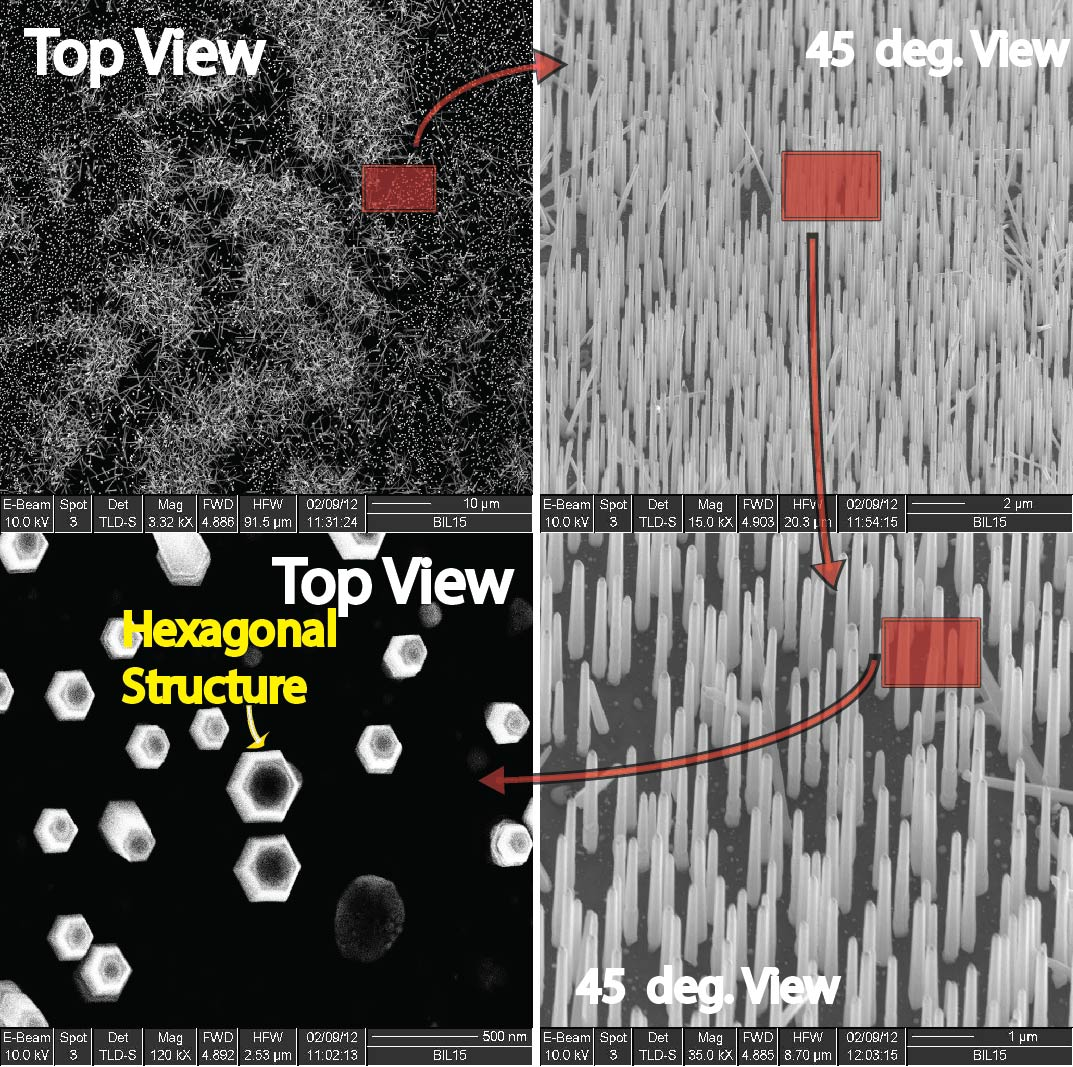
\includegraphics[width=\textwidth]{pictures/Data/SEMNW}
  \label{SEMNW}
\end{figure}

\section{Electrical Characterization of Nanowire}

The as-grown CSNWs are used to perform optical characterization measurement.
However, in order to measure the CSNWs electrical performance, additional
treatments have been taken to make Ohmic contacts between nanowires and
transmission lines.

Characteristic current-voltage (I-V) curves of the nanowire device are given in
Fig.~\ref{CSNWIV_light}. The I-V curve exhibits rectifying behavior, confirming
that the device is a well=behaved diode structure with the electric contact on
one side (Al) ohmic and the other (Pt) Schottky. The reverse bias dark current
of the device is very small, $\sim20pA$ at -1V, and could be further improved
by properly passivating the CSNW surface. Upon illumination, the device shows a
prnounced photovoltaic response due to the built-in potential from the Schottky
junction. The short length of the nanowire device and the large depleted region
by the built-in potential enable the nanowire photodetector to be operated at
zero bias. Fig.~\ref{CSNWIV_light} shows the photocurrent of the device at zero
bias as a function of irradiance. The linearity of the device was demonstrated
up to at least at a 632 nm wavelength. The excellent linear response is in part
based on the good crystalline quality of the nanowires, as confirmed by
transmission electron microscopy. In addition, the capactiance of a typical
device () is calculated to be 5 aF based on a simple parallel-plate model and
thus its cutoff frequency is mainly limited by the transit time of the
photo-generated charge carriers in the device, which may in principle reach ~
100 GHz after certain parameter opti 

\begin{figure}
  \caption{Scanning Electron Microscopy (SEM) image of one dispersed core-shell nanowire connecting with the transmission line by Focus Ion Beam (FIB).}
  \centering
  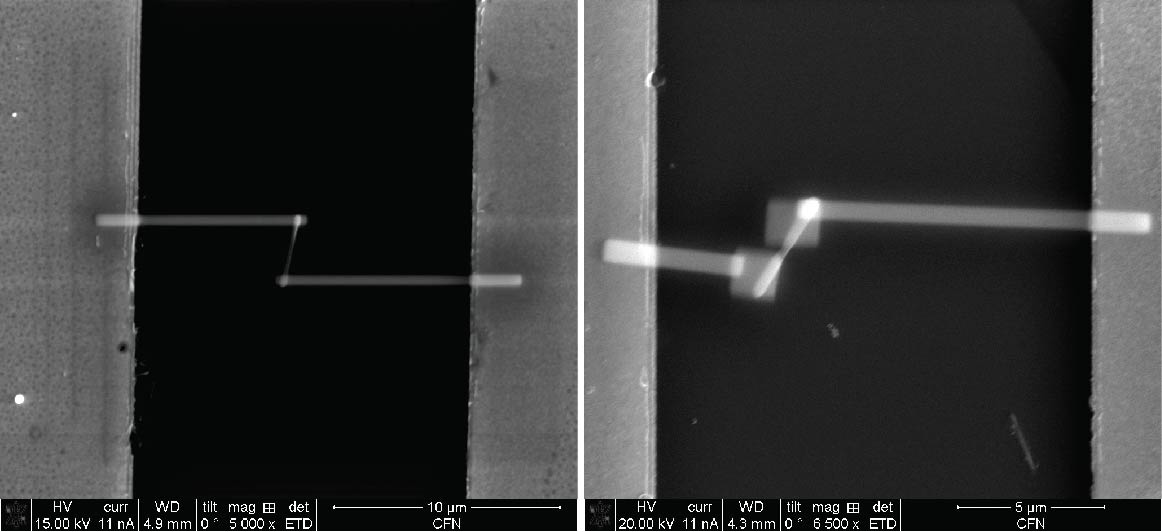
\includegraphics[width=\textwidth]{pictures/Data/ContactNW}
  \label{ContactNW}
\end{figure}

\begin{figure}
  \caption{Current versus Voltage Measurement under illumination of Single Core-Shell Nanowire.}
  \centering
  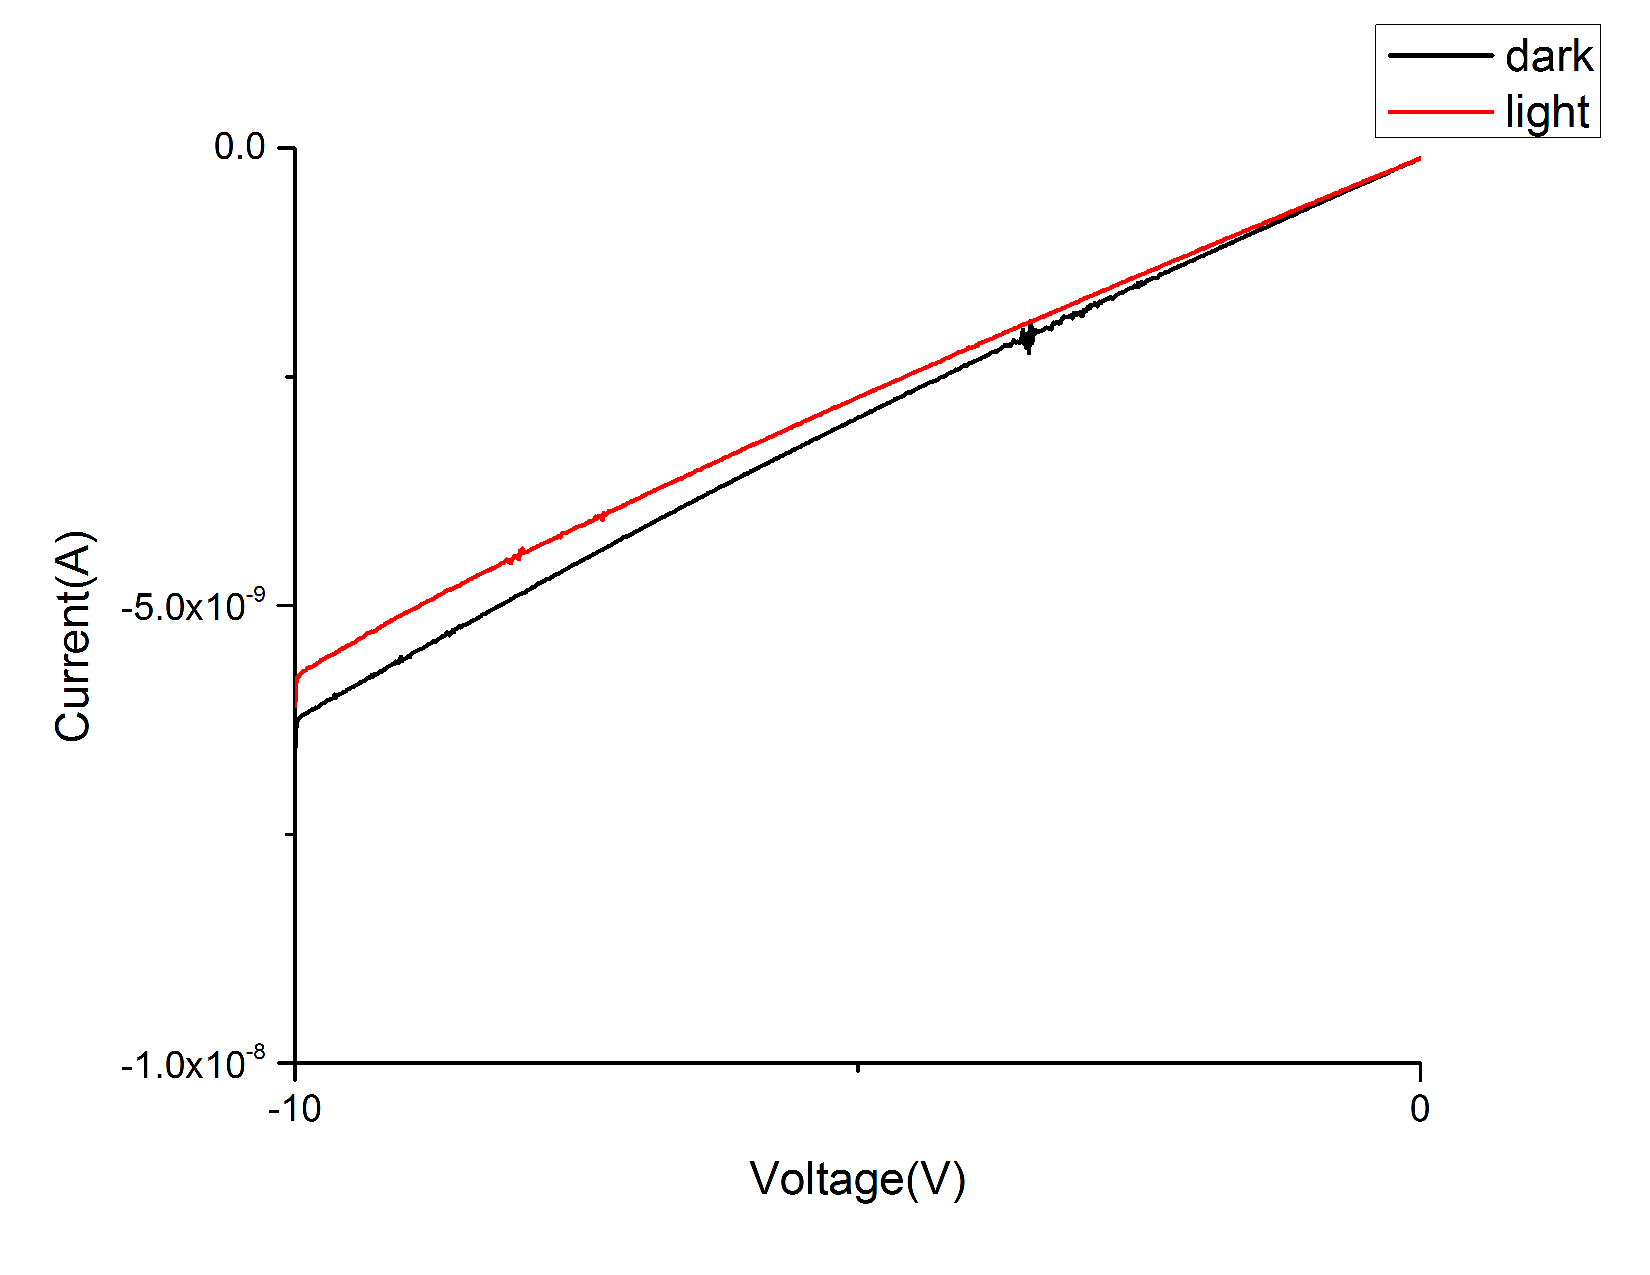
\includegraphics[width=\textwidth]{pictures/Data/CSNWIVlight}
  \label{CSNWIVlight}
\end{figure}

\begin{figure}
  \caption{Capacitance versus Voltage Measurement under illumination of Single Core-Shell Nanowire.}
  \centering
  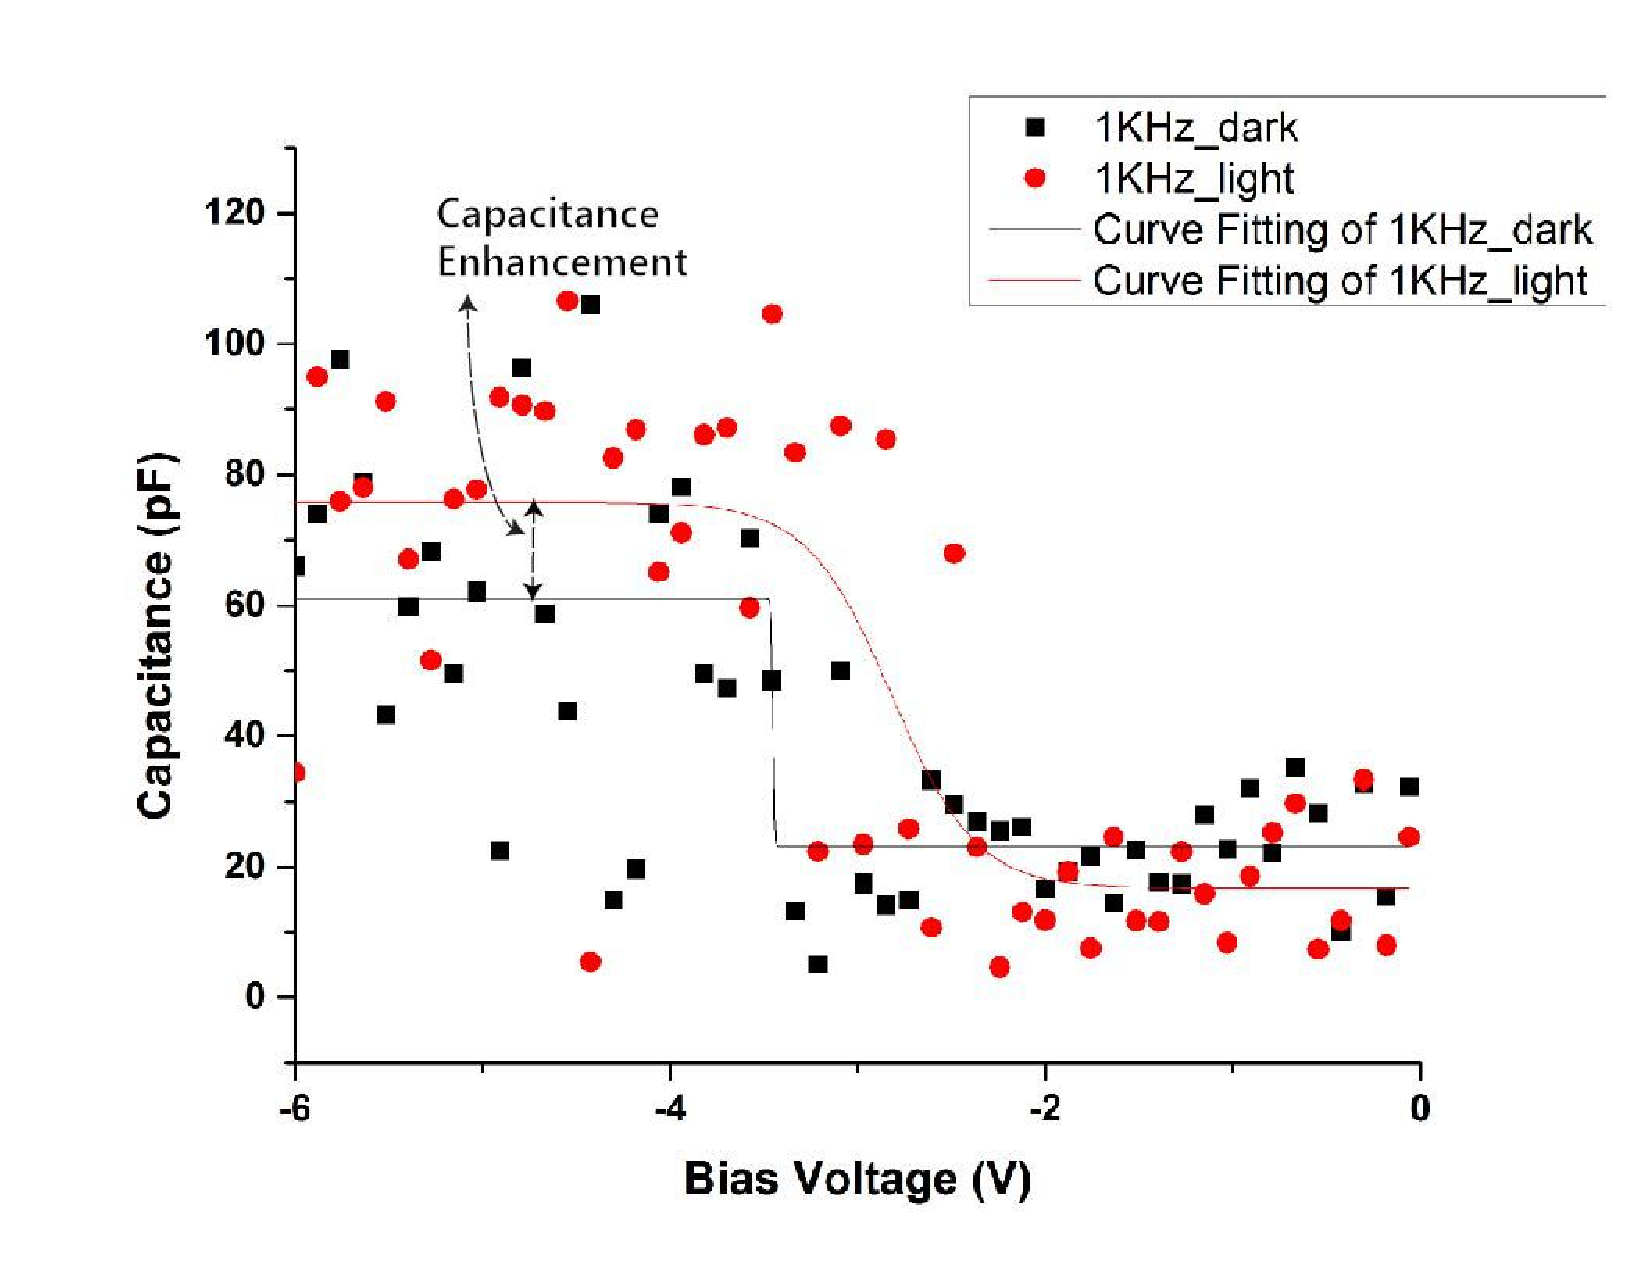
\includegraphics[width=\textwidth]{pictures/Data/CSNWCVlight}
  \label{CSNWCVlight}
\end{figure}

\section{Absorption Enhancement} \label{Data_Abs}

Figure~\ref{reflecbulk} shows the reflectivity of a GaAs wafer on which 50 nm
thin film of AlGaAs is grown, and compared this to the reflectivity spectrum of
a Si substrate. As expected, about 30\% to 55\% of a normally incident light is
reflected in bulk Si and GaAs, with a sharp change for wavelengths near their
respective band gaps. All the data are normalized to the reflectivity of gold
(Au).

\begin{figure}
  \caption{Reflectivity of GaAs (blue) and Si (green) substrates measured with $\sim{\mu}m$ normally incident beam.}
  \centering
  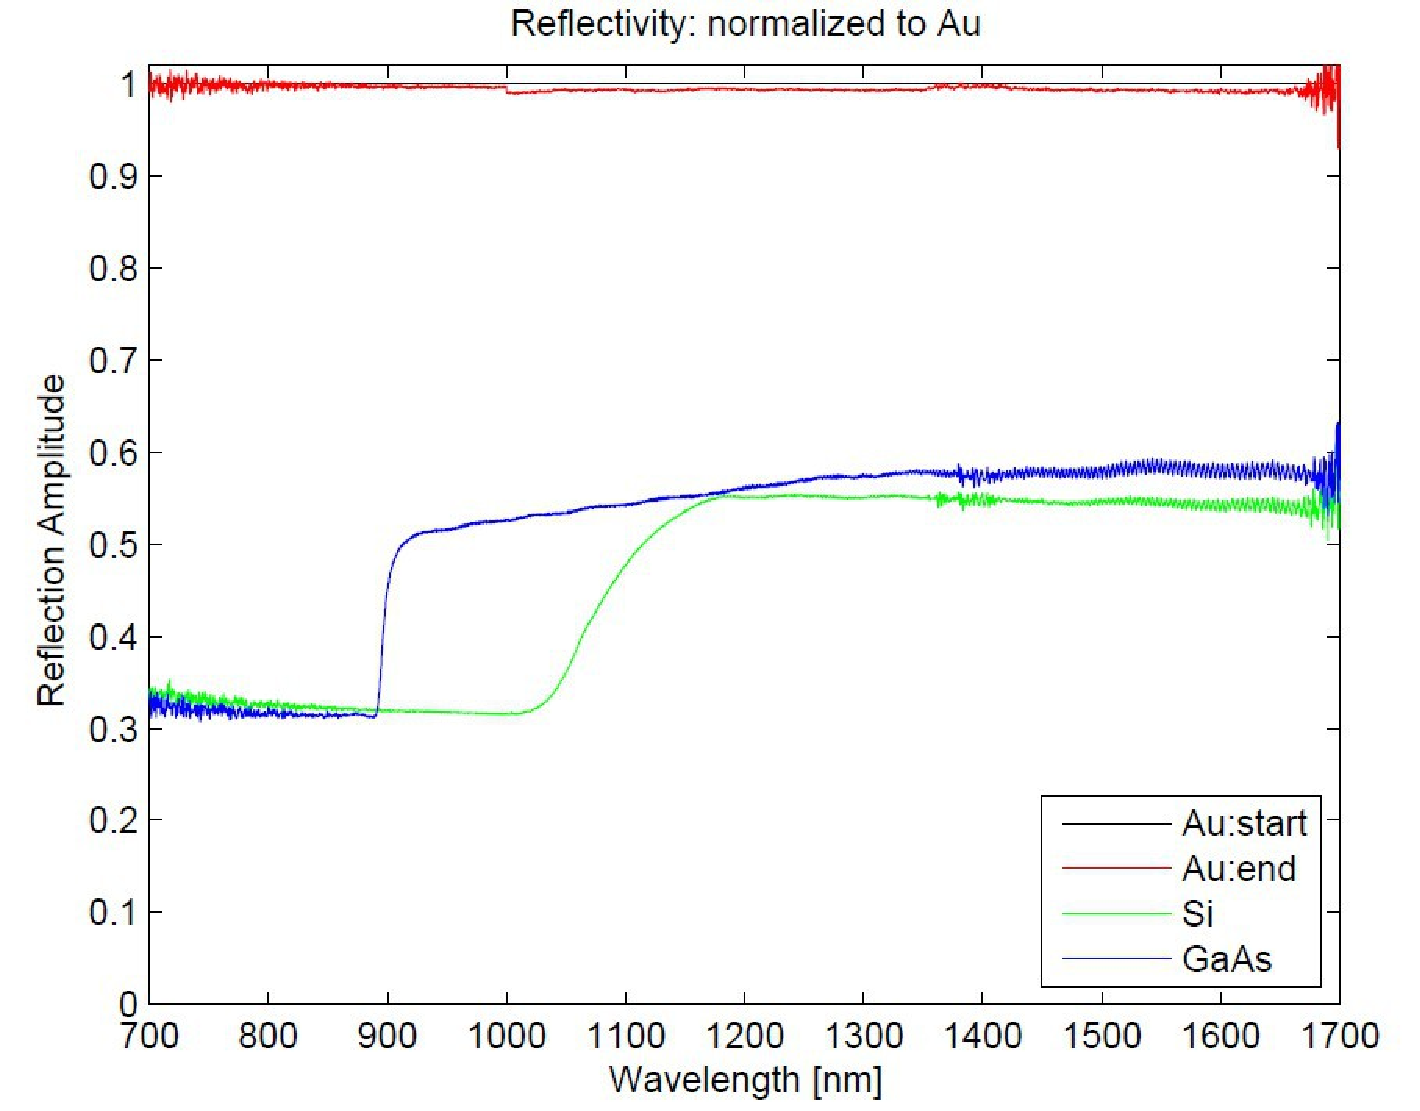
\includegraphics[width=\textwidth]{pictures/Data/reflecbulk}
  \label{reflecbulk}
\end{figure}

Figure~\ref{reflectCSNW} contrasts this with the measured absorption spectrum
of two types of GaAs core, AlGaAs shell nanowires (CSNWs): those grown on a
GaAs substrate (black), and the others heteroexpitaxially grown on a Si
substrate (red). The spectra show that both cases have the signature change of
reflectivity at badgap of GaAs, i.e., these are due to the GaAs/AlGaAs CSNWs,
not the substrate. Importantly, for the wavelength range of 700-1200nm these
core-shells which only occupy ~15\% of the volume compared to thin films of the
same height, reflect 2-4\% of light for the CSNWs grown on Si, and 3-7\% of
light for those grown on GaAs substrate. The beam-width of the incident light
being $\sim1{\mu}m$, this shows that only a few NWs are interrogated by ligth
and, normalized to volume, these wires absorb more than two orders of magnitude
more ligth than their thin-film counterparts.

\begin{figure}
  \caption{Reflectivity spectrum of GaAs/AlGaAs core-shells grown on Si (red) and GaAs (black) substrates shows, normalized to volume, nearly two orders of magnitude more absorption of ligth.}
  \centering
  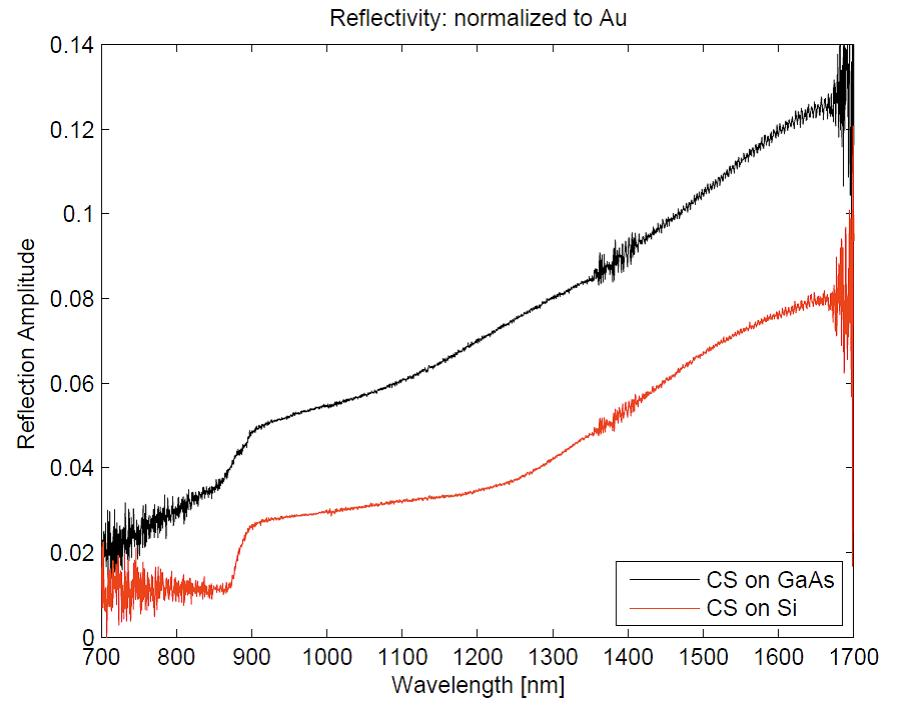
\includegraphics[width=\textwidth]{pictures/Data/reflectCSNW}
  \label{reflectCSNW}
\end{figure}

\section{Emission Enhancement} \label{Dust_data}

Figure~\ref{PL} compares room temperature micro photoluminescence (PL) spectrum
of bulk GaAs to CSNWs grown on GaAs, and two cuts of Si. The ratio of peak
luminescence of a) CSNWs on GaAs, B) CSNWs on Si[111] and c) Si(miscut)
substrates to bulk GaAs are, respectively, 923, 311 and 10. Considering the
beam width of $\sim1{\mu}m$, 5-10 NW were excited, yet emitted over three
order of magnitude more light compared to bulk.

\begin{figure}
  \caption{Photoluminescence of bulk GaAs, Core-Shell Nanowires grown on GaAs and Si.}
  \centering
  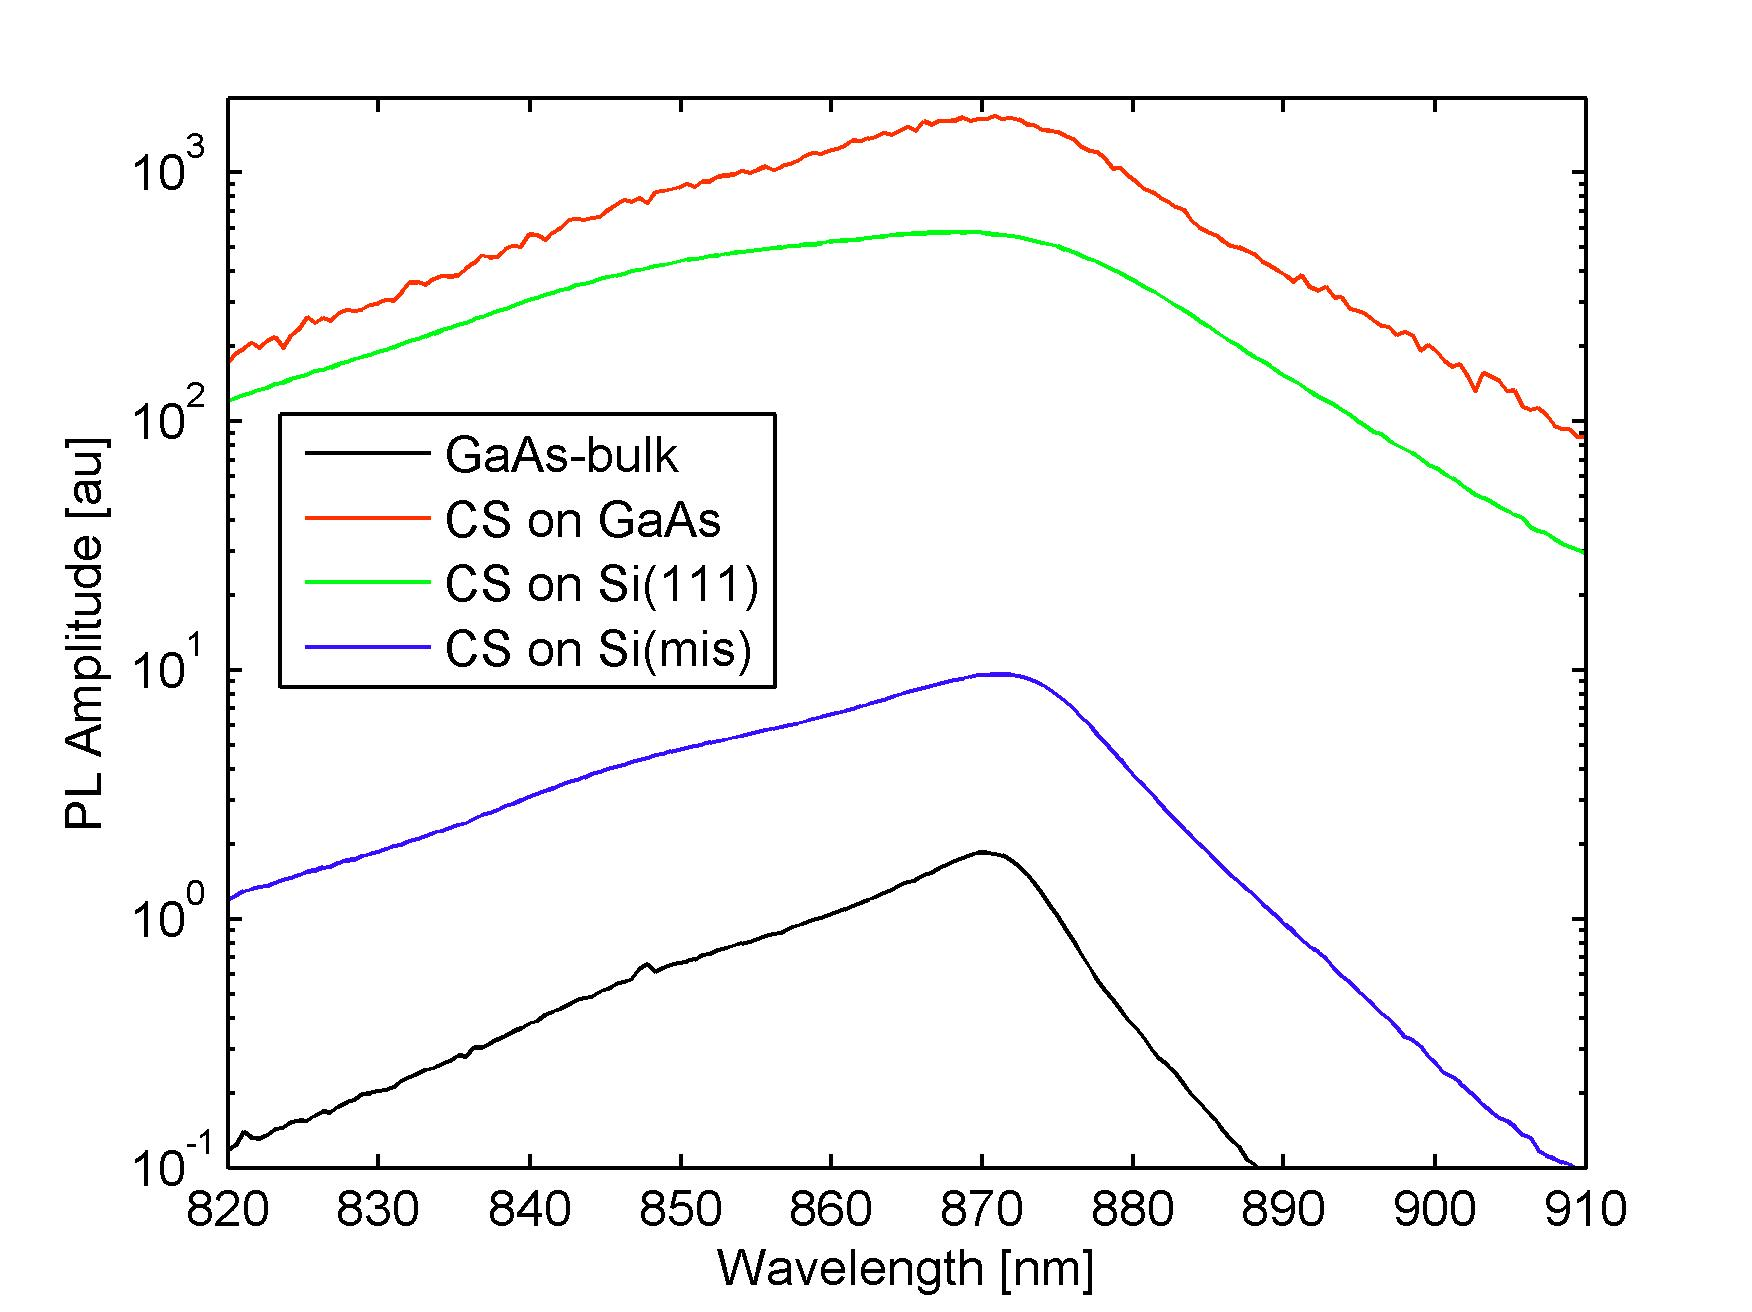
\includegraphics[width=\textwidth]{pictures/Data/PL}
  \label{PL}
\end{figure}

\section{Lasing} \label{data_lasing}

Photoluminescence (PL) of bulk GaAs to CSNWs grown on GaAs, and on two
directions of Si showed that normalized to the fraction of the volume that
these wires occupy, nearly 10,000 times more brightness is observed in these
wires compared to thin-film as in Fig.~\ref{PL}. In the case of stimulated
emission of light, the photon mode density $(1+u_\varepsilon)$ plays a crucial
role. Figure ~\ref{lasing} is the photoluminescence (PL) spectrum at various
optical pump intensities. As the excitation laser power increase beyond
$5{\mu}W$ a sudden and highly nonlinear increase in the emission intensity is
observed, with pronounced peaks emerging from 800nm to 850nm that rapidly grows
to become several orders of magnitude stronger than the background emission.
The lasing amplitude versus excitation power demonstrates a threshold of around
$5{\mu}W$, followed by saturation near $12{\mu}W$. This nonlinear threshold
behavior shows in detail in the L-L plot, (i.e., The pumping power intensity
(L) versus output light power intensity (L)) as in Fig.~\ref{expthreshold}. The
sharp peak has a full width half maximum (FWHM) that varies from 1.5 to 3.5 nm.
This remarkable behavior is achieved in the as-grown wires with no vertical
structure.

\begin{figure}
  \caption{Micro-Photoluminescence measurements with fs-pulsed, 532-nm laser excitation at 250kHz repetition rate shows lasing of the as-grown wires.}
  \centering
  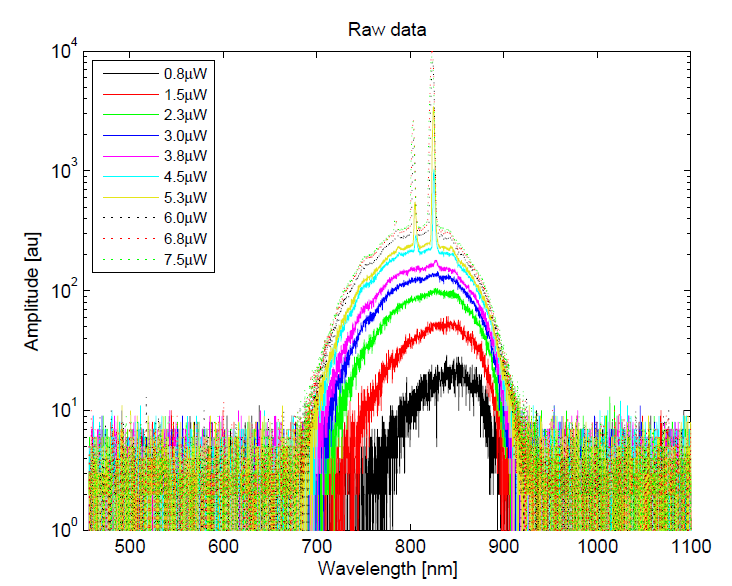
\includegraphics[width=\textwidth]{pictures/Data/lasing}
  \label{lasing}
\end{figure}

\begin{figure}
  \caption{\em{L-L curve of as-grown core-shell nanowire.} The pumping power intensity (L) versus output light power intensity (L) of as-grown core-shell nanowire operating at room temperature with a low threshold of $\sim10{\mu}W$ and followed by saturation near $22{\mu}W$.}
  \centering
  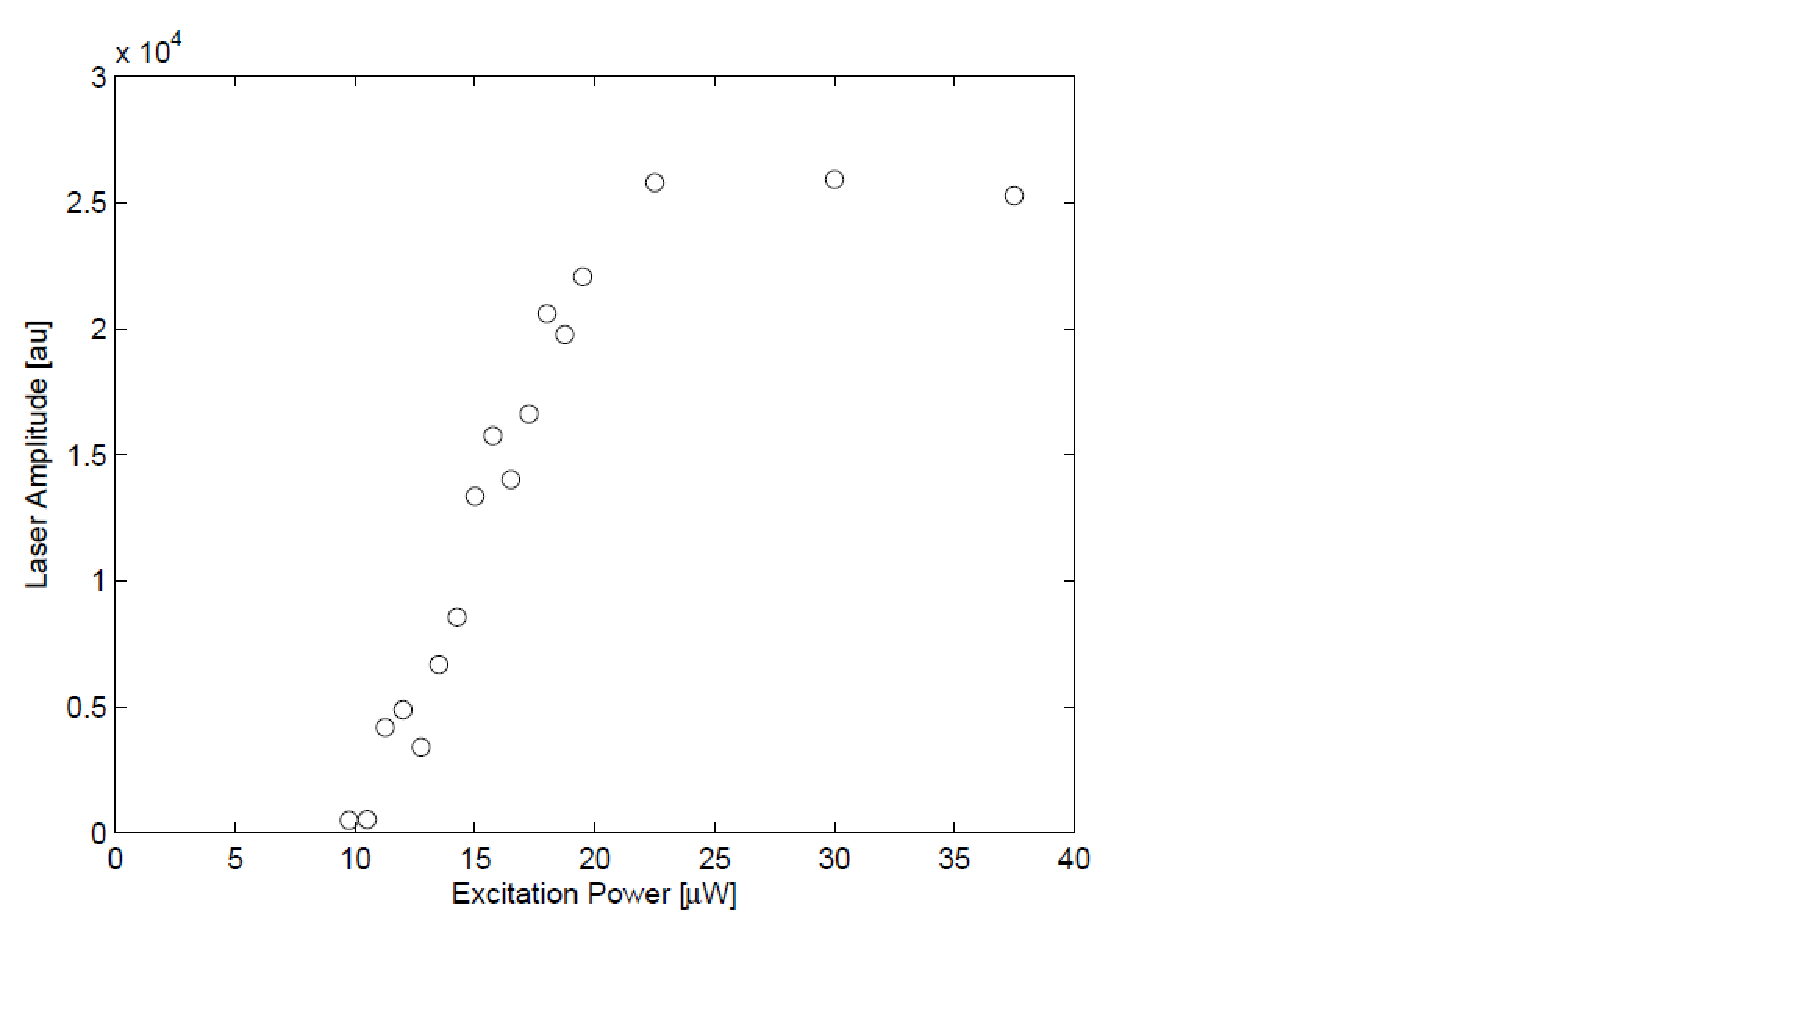
\includegraphics[width=\textwidth]{pictures/Data/expthreshold}
  \label{expthreshold}
\end{figure}
